\subsection{Dynamics results}
\label{subsec:molecular_dynamics_results}

Figure~\ref{fig:high_density_system_evolution} shows time evolution of a high density system. The in the low temperature regime (Figure~\ref{fig:high_density_system_evolution:low_t}) the system is frozen and doesn't have energy to overpower potential barrier, therefore we see many small clusters of particles. Also the system is far from equilibrium. \textcolor{red}{add same figure for MC evolution?} The most organised is the system with average value of $k_BT = 1$ (Figure~\ref{fig:high_density_system_evolution:mid_t}). In the high temperature case (Figure~\ref{fig:high_density_system_evolution:high_t}), the particle cluster are the most fluid and change its orientation easily.

\begin{figure}[h]
\centering
\begin{subfigure}[t]{0.29\textwidth}
	\centering
	\includegraphics[height=4.5cm]{Images/Picture_Data_2.png}
	\captionsetup{justification=centering, width=0.9\columnwidth}
	\caption{$k_BT = 0.5$}
	\label{fig:high_density_system_evolution:low_t}
\end{subfigure}
\begin{subfigure}[t]{0.29\textwidth}
	\centering
	\includegraphics[height=4.5cm]{Images/Picture_Data_3.png}
	\captionsetup{justification=centering, width=0.9\columnwidth}
	\caption{$k_BT = 1$}
	\label{fig:high_density_system_evolution:mid_t}
\end{subfigure}
\begin{subfigure}[t]{0.29\textwidth}
	\centering
	\includegraphics[height=4.5cm]{Images/Picture_Data_4.png}
	\captionsetup{justification=centering, width=0.9\columnwidth}
	\caption{$k_BT = 2$}
	\label{fig:high_density_system_evolution:high_t}
\end{subfigure}
\begin{subfigure}[t]{0.1\textwidth}
	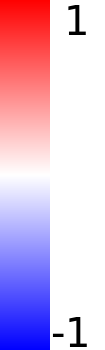
\includegraphics[height=4.5cm, right]{Images/gradient.png}
\end{subfigure}
\captionsetup{justification=centering, width=0.9\columnwidth}
\caption{Langevin Dynamics simulation of system evolution for different temperature. The simulation runs from state where all particles are randomly oriented at $t = 0$ to $t = 10^3$. Time evolution goes from bottom to top. Black area is absence of a particle, and color shows value of $\cos \theta$. The simulations are performed for $N = 1000$ particles and $\rho = 0.95$}
\label{fig:high_density_system_evolution}
\end{figure}

Next we looked into relaxation order parameter to its equilibrium value. For that we made Langevin dynamics simulations for the selected values of $k_BT = (0.6, 0.8, 1, 1.6)$ and density $\rho = (0.25, 0.5, 0.95)$, again for two different system sizes of $N = (800, 1600)$ particles. The obtained results are shown on the figure
%~\ref{fig:order_parameter_relaxation}.

%\begin{figure}[h]
%\centering
%	\begin{subfigure}{0.29\textwidth}
%		\centering
%		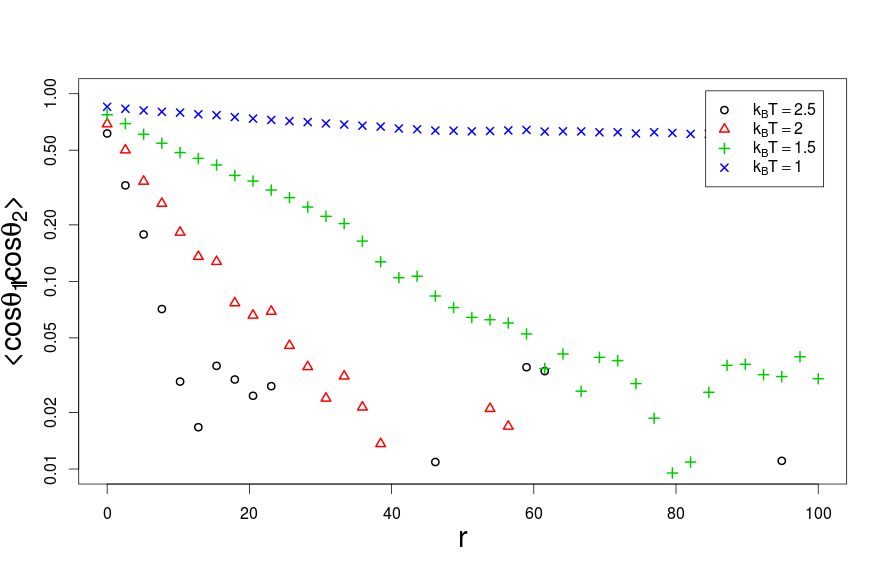
\includegraphics[width=0.9\textwidth]{Images/corr_5k_095.png}
%		\captionsetup{justification=centering, width=0.9\columnwidth}
%		\caption{$\rho = 0.25$}
%		\label{fig:op_from_coaligned}
%	\end{subfigure}
%	\begin{subfigure}{0.29\textwidth}
%		\centering
%		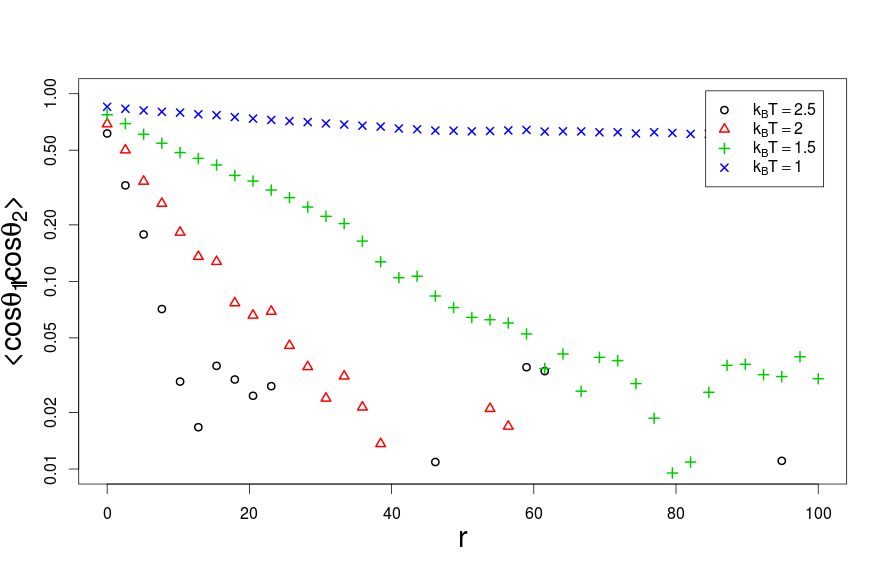
\includegraphics[width=0.9\textwidth]{Images/corr_5k_095.png}
%		\captionsetup{justification=centering, width=0.9\columnwidth}
%		\caption{$\rho = 0.5$}
%		\label{fig:op_from_coaligned}
%	\end{subfigure}
%	\begin{subfigure}{0.29\textwidth}
%		\centering
%		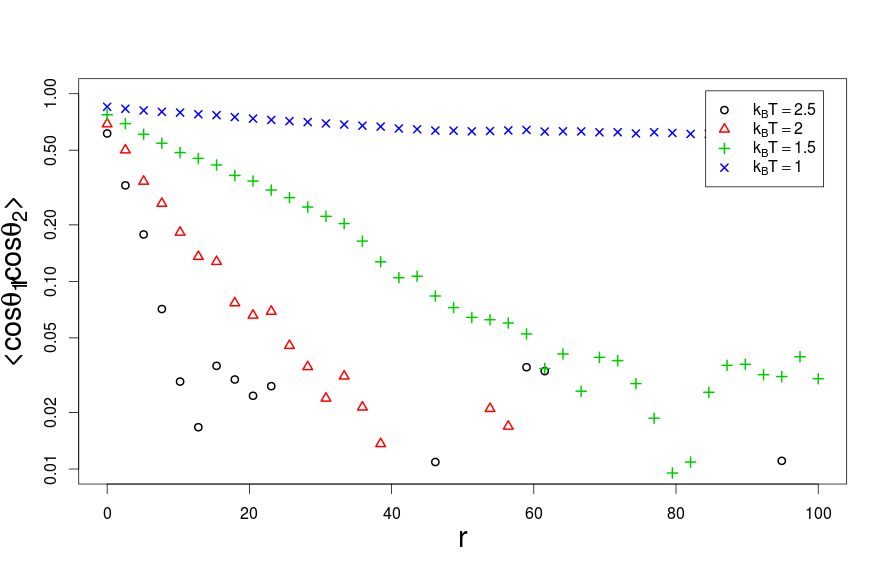
\includegraphics[width=0.9\textwidth]{Images/corr_5k_095.png}
%		\captionsetup{justification=centering, width=0.9\columnwidth}
%		\caption{$\rho = 0.95$}
%		\label{fig:op_from_coaligned}
%	\end{subfigure}
%	\captionsetup{justification=centering, width=0.9\columnwidth}
%	\caption{Equilibrium orientation correlation as function of distance for different values of density and $k_BT$. Simulations were done for $N = 5000$ particles, and were averaged over $200$ samples}
%	\label{fig:order_parameter_relaxation}
%\end{figure}